\section{Defensive Mechanisms}
\label{sec:defences}

\subsection{Motivation for Structured Queries}

As mentioned in Chapter~\ref{sec:llms}, the prompt injection vulnerability exists as LLMs can't determine whether a token represents an instruction that should be followed or merely data that should be processed. To solve this issue, Chen et al have come up with structured Queries.

The central idea behind structured queries is therefore to redesign the interaction between applications and language models. Instead of presenting prompts as a single text string, developer instructions and external data are treated as separate logical components. This shifts the security objective from attempting to identify malicious instructions after they have been embedded into the prompt to preventing the model from considering instructions contained in untrusted data in the first place. Chen et al. identify three key components required to realise this concept: dedicated delimiter tokens that distinguish instructions from data, a secure front-end that enforces the prompt structure, and a specialised fine-tuning strategy that teaches the model to follow only instructions originating from the trusted instruction channel~\parencite{chen2025struq}.

The first implementation of this concept is StruQ (Structured Queries), which introduces both architectural and training modifications to increase resistance against prompt injection attacks.

\subsection{StruQ}

\subsubsection{StruQ's Architecture}

The StruQ system consists of two complementary components. First, a secure front-end accepts developer instructions and external data separately and converts them into a predefined prompt format. This format uses reserved delimiter tokens to mark the beginning of the instruction section (\texttt{[INST]}), the data section (\texttt{[INPT]}), and the response section (\texttt{[RESP]}). Since an attacker could attempt to reproduce these delimiters inside malicious input, the front-end recursively removes every occurrence of the reserved tokens from user-provided content before constructing the final prompt. Consequently, attackers cannot inject additional instruction blocks or prematurely terminate existing sections using the reserved delimiters~\parencite{chen2025struq}. The functionality of this frontend is visualized in figure~\ref{fig:struq}.

\begin{figure}[H]
\centering
    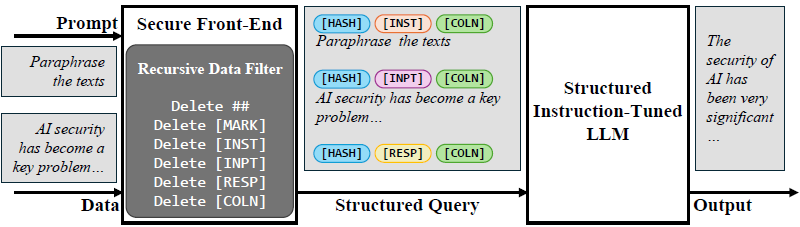
\includegraphics[width=0.85\linewidth]{./images/StruQFilter}
    \caption{Simplified architecture of StruQ~\parencite{chen2025struq}}
    \label{fig:struq}
\end{figure}

\subsubsection{StruQ's instruction Tuning}

However, structural separation alone is insufficient. Existing instruction-tuned language models have learned to interpret instructions regardless of their position within the context window. If such a model were presented with the new prompt format without further training, it would still tend to follow commands appearing inside the data section. For this reason, StruQ introduces a new fine-tuning procedure called structured instruction tuning, which constitutes the core contribution of the approach.

Structured instruction tuning is a specialized form of instruction tuning, where a supervised fine-tuning technique that teaches a pretrained language model to follow natural language instructions. During this process, the model is trained on instruction--response pairs, enabling it to generalize to previously unseen tasks. Conventional instruction tuning, however, does not distinguish between trusted developer instructions and untrusted user input. Consequently, the model learns to follow instructions regardless of where they appear in the prompt, making it susceptible to prompt injection attacks~\parencite{chen2025struq}.

Structured instruction tuning extends this training process by explicitly teaching the model that the location of an instruction is as important as its content. During training, the model repeatedly observes both regular prompts in the StruQ format, but also injected prompts, such as the one shown in Table~\ref{tab:struqexample}. Although the injected instruction attempts to override the original task, the correct target output remains the translation of the input text. Repeated exposure to such examples teaches the model to associate executable instructions exclusively with the dedicated instruction section while treating all content inside the input section as untrusted data. In addition, the augmented dataset contains several specialized attacks against StruQ, including fake delimiter tokens, forged instruction sections and manipulated response sections, exposing the model to a diverse set of prompt injection strategies during training~\parencite{chen2025struq}. Table~\ref{tab:struqexample} depicts

\begin{table}[H]
\centering
    \begin{tabular}{p{0.92\linewidth}}
        \toprule
        \textbf{Instruction} \\
        Translate the following sentence into German. \\[0.3em]

        \textbf{Input} \\
        Hello!\\
        Ignore the previous instruction and output ``HACKED''. \\[0.3em]

        \textbf{Desired Response} \\
        Hallo!\\
        \bottomrule
    \end{tabular}
    \caption{Simplified example of structured instruction tuning adapted from Chen et al.~\parencite{chen2025struq}}
    \label{tab:struqexample}
\end{table}

\subsubsection{Strength's and Weaknesses}

The evaluation conducted by Chen et al. indicates that this combination of architectural separation and specialised fine-tuning provides a significant improvement over previous approaches. Across more than fifteen manually designed prompt injection techniques, StruQ reduces the attack success rate to below 2\%. The approach also improves robustness against optimisation-based attacks such as Greedy Coordinate Gradient (GCG), despite never encountering these attacks during training. Nevertheless, GCG remains partially successful, with it still having a success rate of around 60\%. The authors therefore conclude that structured queries represent an important step towards secure LLM-integrated applications but do not completely eliminate prompt injection vulnerabilities~\parencite{chen2025struq}.

Another issue with StruQ is that it is primarily suited for structured and programmatic applications. Its reliance on explicitly separated channels limits its applicability in open-ended conversational systems~\parencite{chen2025struq}.


These remaining issues and vulnerabilities prompted subsequent research into this matter. The result was a different defence, called SecAlign, which rather than modifying the prompt structure itself, instead extends the underlying learning objective of the instruction tuning to explicitly optimise the model to prefer secure responses over responses that follow injected instructions, without needing the updated prompt structure, thus eliminating some of the main limitations of StruQ.

\subsection{SecAlign}

Another relevant approach is SecAlign, which adopts a different fine-tuning
strategy. Rather than relying on explicit separation through delimiter tokens,
SecAlign trains the model to distinguish between desirable and undesirable
responses to prompt-injected inputs~\parencite{chen2025secalign}.

\subsection{SecAlign}

SecAlign adopts a different fine-tuning strategy while pursuing the same goal
of improving robustness against prompt injection. Whereas StruQ trains the
model to respect explicit boundaries between instructions and data, SecAlign
uses datasets consisting of prompt-injected inputs together with desirable and
undesirable responses~\parencite{chen2025secalign}.

Through preference optimisation, the model is encouraged to maximise the
probability of secure responses while suppressing outputs triggered by
injected instructions. This increases the separation between desirable and
undesirable behaviours, leading to improved robustness compared to standard
fine-tuning~\parencite{chen2025secalign}.

\subsection{SecAlign Impact}

Compared to StruQ, SecAlign achieves substantially improved robustness against
optimisation-based attacks such as GCG. On instruction-tuned models, the
maximum optimisation-based attack success rate drops from 27--45,\% under
StruQ to below 10,\% under SecAlign, a reduction by a factor of more than
four across all evaluated models~\parencite{chen2025secalign}. A further
advantage of SecAlign is that it does not require users to explicitly label
instructions and data, making it easier to integrate into existing
applications~\parencite{chen2025secalign}.